\documentclass{article}
\usepackage[utf8]{inputenc}
\usepackage[T1]{fontenc}
\usepackage{booktabs}
\usepackage{xcolor}
\usepackage{fontawesome5}
\usepackage{geometry}
\usepackage{array}
\usepackage{helvet}
\usepackage{titlesec}
\usepackage{parskip}
\usepackage{mdframed}
\usepackage{hyperref}
\usepackage{ragged2e}
\usepackage{graphicx}
\usepackage{ccicons}
\usepackage{fancyhdr}
\usepackage{lmodern}
\usepackage[export]{adjustbox}

% Meta-Informationen für den PDF-Export
\hypersetup{
    pdftitle={Kursimport vs. Zwischenspeicher},
    pdfauthor={Christian-Maximilian Steier},
    pdfsubject={Vergleich von Kursimport und Zwischenspeicher in Moodle},
    pdfkeywords={Moodle, Kursimport, Zwischenspeicher, Christian-Maximilian Steier},
    colorlinks=true,
    linkcolor=customred,
    urlcolor=customred,
    pdfborderstyle={/S/U/W 1}
}

\renewcommand{\familydefault}{\sfdefault}

% Keine Worttrennung
\tolerance=1
\emergencystretch=\maxdimen
\hyphenpenalty=10000
\hbadness=10000
\raggedright

\geometry{a4paper, margin=2.5cm}
\definecolor{customred}{RGB}{230, 0, 40}
\definecolor{lightred}{RGB}{255, 235, 238}
\definecolor{lightgray}{RGB}{245, 245, 245}
\definecolor{ccboxborder}{RGB}{200, 200, 200}
\definecolor{ccboxbg}{RGB}{245, 245, 245}

% Titelgestaltung
\titleformat{\section}
  {\normalfont\Large\bfseries\color{customred}}
  {}{0em}{}[\vspace{-0.5em}\rule{\textwidth}{0.5pt}]

% Fußzeile
\pagestyle{fancy}
\fancyhf{}
\renewcommand{\headrulewidth}{0pt}
\fancyfoot[C]{
\ccby{}\quad Dieses Dokument wurde erstellt von \textbf{ZWEK} der Hochschule Düsseldorf und steht unter der Lizenz \textbf{CC BY 4.0}.  
Weitere Informationen: \url{https://creativecommons.org/licenses/by/4.0/}\\
\textsf{\small{Stand: April 2025 • Moodle Version 4.5}}}

% Gemeinsame Breite
\newlength{\commonwidth}
\setlength{\commonwidth}{16cm}

% Modernisierte CC-Box
\newenvironment{ccbox}{%
  \begin{center}
  \begin{minipage}{\commonwidth}
  \begin{mdframed}[
    backgroundcolor=ccboxbg,
    linecolor=ccboxborder,
    linewidth=0.8pt,
    roundcorner=5pt,
    leftmargin=0pt,
    innerleftmargin=1em,
    innerrightmargin=1em,
    innertopmargin=0.7em,
    innerbottommargin=0.7em
  ]
  \centering
  \small
}{%
  \end{mdframed}
  \end{minipage}
  \end{center}
}

\begin{document}

% Titel
\begin{center}
\textbf{\textcolor{customred}{\LARGE Kursimport \faFileImport{} vs. Zwischenspeicher \faShoppingCart}}
\end{center}

\vspace{0.5cm}

% Usecase Box
\begin{center}
\begin{minipage}{\commonwidth}
\begin{mdframed}[backgroundcolor=lightgray, linewidth=0pt, roundcorner=5pt]
\textbf{Anwendungsfall:}

Sie beginnen ein neues Semester und möchten bewährte Inhalte aus alten Kursen weiterverwenden.

\vspace{0.3cm}

\textbf{Szenarien:}
\begin{itemize}
  \item \textbf{Kursimport:} Um den gesamten Kurs oder große Teile (inkl. Aktivitäten, Fragenpools etc.) zu übernehmen.
  \item \textbf{Block "Zwischenspeicher zum Teilen":} Gezielt einzelne Inhalte wie Videos, Aufgaben oder Materialien in mehreren wiederverwenden.
\end{itemize}
\end{mdframed}
\end{minipage}
\end{center}

\vspace{0.8cm}

\renewcommand{\arraystretch}{1.4}  % Erhöht den Zeilenabstand in der Tabelle
\setlength{\tabcolsep}{8pt}        % Setzt den Spaltenabstand

% Tabelle zentriert mit linksbündigem Text in den Zellen
\begin{center}
\begin{minipage}{\commonwidth}
\begin{tabular}{>{\bfseries\raggedright\arraybackslash}p{3.5cm}>{\raggedright\arraybackslash}p{6cm}>{\raggedright\arraybackslash}p{6cm}}
\toprule
\textcolor{customred}{\textbf{}} 
& \textbf{Kursimport \faFileImport} 
& \textbf{Zwischenspeicher \faShoppingCart} \\
\midrule
Inhalt & \faLayerGroup~Komplette Kurse oder größere Abschnitte 
       & \faCubes~Einzelne Materialien oder Aktivitäten \\
\midrule
Voraussetzung 
       & \faUserTie~Lehrenden-Rolle in beiden Kursen 
       & \faPuzzlePiece~Plugin „Zwischenspeicherzum Teilen" muss installiert sein \\
\midrule
Zugriff & \faCogs~Kursnavigation Mehr → Kurse wiederverwenden  → Import 
        & \faToggleOn~Block „Zwischenspeicher zum Teilen" anlegen \\
\midrule
Quellkurs & \faBook~Nur ganze Kurse auswählbar 
          & \faUniversalAccess~Einzelne Elemente aus beliebigen Kursen \\
\midrule
Zielkurs & \faArrowRight~Import in gesamten Kurs 
         & \faRandom~Einfügen in beliebige Kursbereiche \\
\midrule
Struktur & \faSitemap~Übernimmt Struktur des Quellkurses 
         & \faFolder~Eigene Ordnung im Zwischenspeicher möglich \\
\midrule
Nutzerdaten & \faUsersCog~Mit oder ohne Nutzerdaten (nicht empfohlen) 
            & \faUserSlash~Keine Nutzerdaten werden übertragen \\
\midrule
Typische Nutzung & \faCalendarCheck~Zu Beginn des Semesters 
                 & \faSync~Während des Semesters flexibel nutzbar \\
\midrule
Zeitaufwand & \faHourglassHalf~Mittel (mehrere Schritte) 
            & \faHandPointer~Gering (per Drag \& Drop) \\
\midrule
Geeignet für & \faClone~Komplette Kurse erneut verwenden 
                       & \faLightbulb~Kleinere Inhalte/Aktivitäten übertragen \\
\bottomrule
\end{tabular}
\end{minipage}
\end{center}

\vspace{0.7cm}

% Tipp-Box zentriert mit gleicher Breite wie die Tabelle
\begin{center}
\begin{minipage}{\commonwidth}
\fcolorbox{customred!30}{lightred!30}{%
    \begin{minipage}{\dimexpr\commonwidth-2\fboxsep-2\fboxrule}
    \raggedright % Inhalt der Box linksbündig
    \textbf{\textcolor{customred}{Tipp:}} Kombinieren Sie beide Methoden! Verwenden Sie den Kursimport zu Semesterbeginn für die Grundstruktur und den Zwischenspeicher für spezifische Inhalte während des Semesters.
    \end{minipage}%
}
\end{minipage}
\end{center}

\vspace{1.5cm}

\begin{figure}
    \centering
    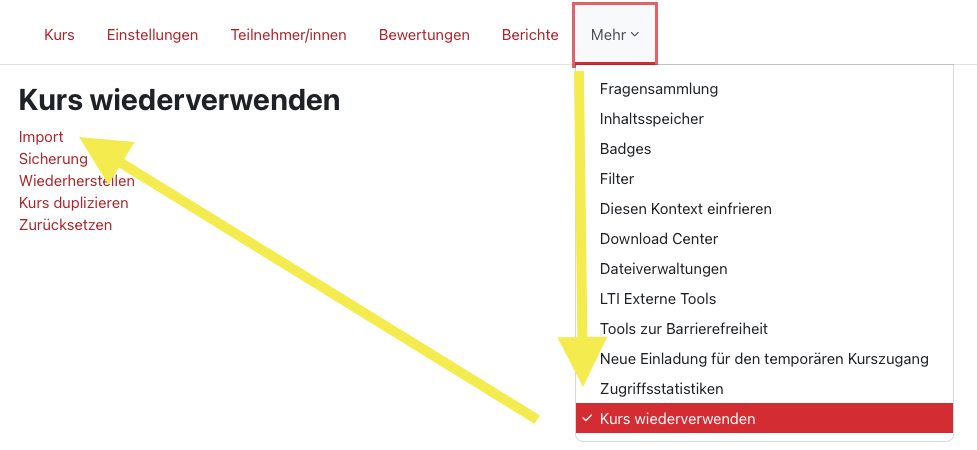
\includegraphics[width=0.48\textwidth]{Bilder/Bild1.png}
    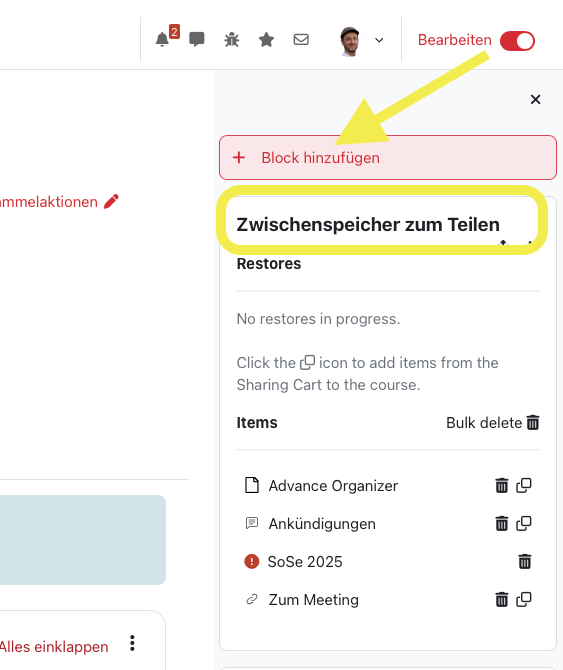
\includegraphics[width=0.48\textwidth]{Bilder/Bild2.png}
\end{figure}

\vspace{3.5cm}

% Literatur und Links Box zentriert
\begin{center}
\begin{minipage}{\commonwidth}
\begin{mdframed}[
    backgroundcolor=lightgray, 
    linewidth=0pt, 
    roundcorner=5pt,
    innerleftmargin=1em,
    innerrightmargin=1em,
    innertopmargin=0.7em,
    innerbottommargin=0.7em
]
\raggedright % Inhalt der Box linksbündig
\textbf{\textcolor{customred}{Literatur \& Links zum Thema}}
\vspace{0.2cm}

\begin{itemize}
\item \textbf{Offizielle Moodle-Dokumentation:}
\vspace{0.2cm}
  \begin{itemize}
  \item Kursimport: \url{https://docs.moodle.org/de/Kursdaten_importieren}
  \item Sharing Cart / Zwischenspeicher: \url{https://docs.moodle.org/en/Sharing_Cart}
  \end{itemize}
\vspace{0.5cm}

\item \textbf{Video-Tutorials:}
\vspace{0.2cm}
  \begin{itemize}
  \item Import: Kurse und Inhalte kopieren: \url{https://youtu.be/E4vCJYTllLg?si=vP_mQVyX4CvrcKp9}
  \item Materialkoffer: Inhalte sammeln und kopieren: \url{https://youtu.be/FWIpteXKMVI?si=cxFFoWs6YP_NQyxm}
  \end{itemize}
\end{itemize}
\end{mdframed}
\end{minipage}
\end{center}

\vspace{1cm}

\end{document}
